\documentclass{article}


\usepackage{arxiv}

\usepackage{placeins}
\usepackage[utf8]{inputenc} % allow utf-8 input
\usepackage[T1]{fontenc}    % use 8-bit T1 fonts
\usepackage{hyperref}       % hyperlinks
\usepackage{url}            % simple URL typesetting
\usepackage{booktabs}       % professional-quality tables
\usepackage{amsfonts}       % blackboard math symbols
\usepackage{nicefrac}       % compact symbols for 1/2, etc.
\usepackage{microtype}      % microtypography

\usepackage{graphicx}	% to insert graphs
\usepackage{caption}	% to customize caption style
\usepackage{float}
\usepackage{subfigure}


\title{Predicting the OutcomHASe of 2020 English Premier League (EPL) Football Matches}


\author{
 Group Name: \texttt{Group D}\\
  Department of Computer Science\\
  University College London\\
  London, WC1E 6BT\\
}


\begin{document}

\maketitle
\captionsetup[figure]{labelformat={default},labelsep=period,name={Fig.}}


% -------------------------------------------------------------------------------------------
\section{Introduction }


% -------------------------------------------------------------------------------------------
\section{Data Transformation \& Exploration}

At first sight, we found that:
\begin{itemize}
\item The shape of the data frame is 4180 rows x 73 columns, but some columns are empty and unnamed.
\item There are two different date formats, "\%d\/\%m\/\%y" and "\%d\/\%m\/\%Y".
\item The involved data is from 2008-08-16 to 2019-05-12 (i.e. totally 11 seasons).
\end{itemize}

\begin{figure}[ht]
\centering
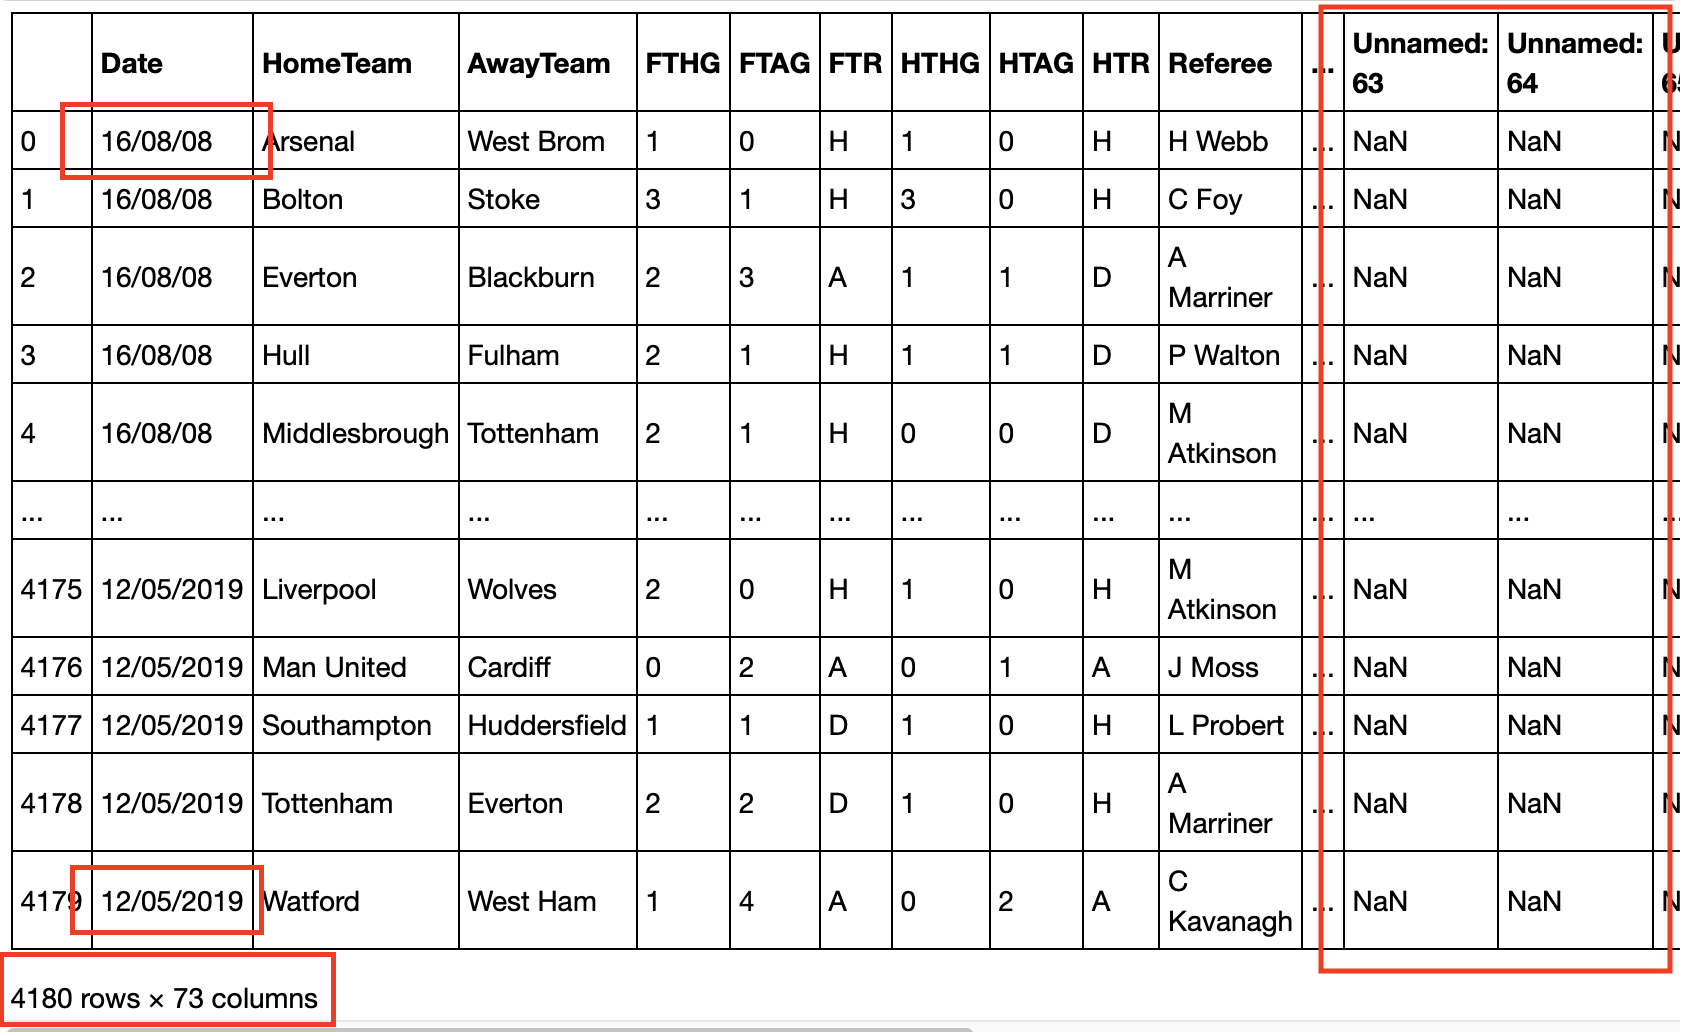
\includegraphics[scale=0.4]{graphs/firstSight.png}
\caption{ First sight of training data}
\label{fig:firstSight}
\end{figure}

% -------------------------------------------------------
\subsection{Data Cleaning}

After we dropped the unnamed columns, the number reduced to 22.

We verified that there is no row containing invalid values (i.e., None, NaN, infinite or overflowed number), so we don’t need to drop any rows. The size remains 4180.

We then unified the date formats, converting into “\%Y-\%m-\%d” for later exploration and transformation.
% -------------------------------------------------------
\subsection{Initial Data Exploration}
% ----------------------------
\subsubsection{Number of matches per season}
The full set is of huge amount. To help learn the data, we separated rows by date from August to May (i.e., one season) to check how many matches there are per season.
\begin{figure}[ht]
\centering
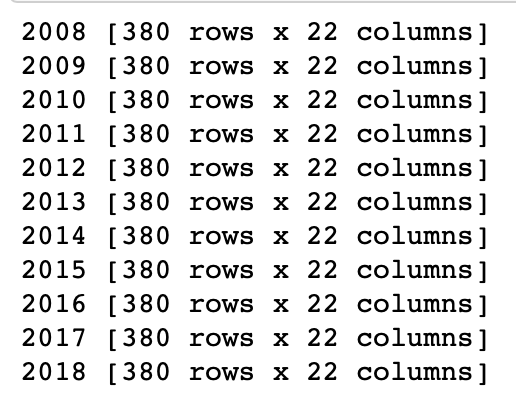
\includegraphics[scale=0.6]{graphs/matchesPerSeason.png}
\caption{Number of matches per season}
\label{fig:matchesPerSeason}
\end{figure}

We found that the number of matches each season stays constant (380).

% ----------------------------
\subsubsection{Relationship between attributes}
We plotted a Pearson Correlation Heatmap (Fig. \ref{fig:top-10-features-in-raw-data}) to see the top 10 features related to the match result (FTR).

\begin{figure}[ht]
\centering
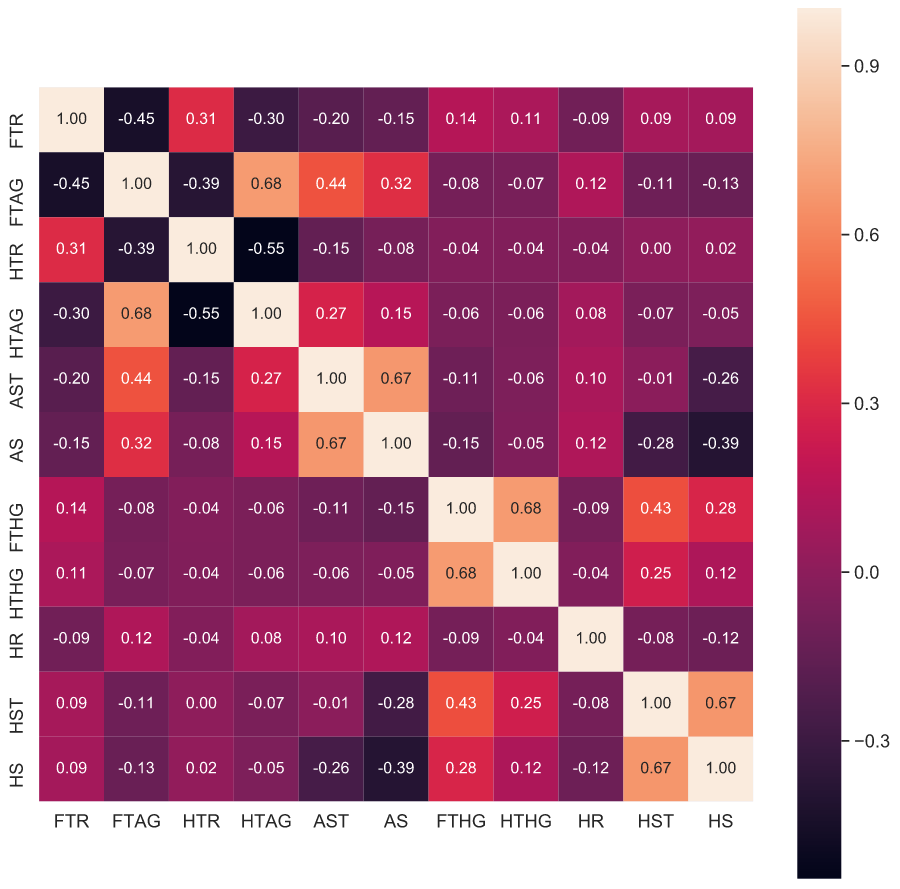
\includegraphics[scale=0.3]{graphs/top-10-features-in-raw-data.png}
\caption{The top 10 features related to FTR}
\label{fig:top-10-features-in-raw-data}
\end{figure}

As shown in the graph, the top 10 features are: \\
\centerline{HTR,  FTHG, HTHG, HST, HS, HR, AS, AST, HTAG, FTAG,}	\\
ordered from the greatest to least.

It is notable that the goal scored at full time (FTHG, FTAG)  \& goal scored at half time (HTHG, HTAG) and
the total number of shots on goal (HS, AS)  \& that on target (HST, AST) are the two pairs of data which are highly correlated (> 0.65).

% -------------------------------------------------------
\subsection{Feature Construction}
So, within the top 10 we picked FTHG, FTAG , HS, AS,  HR, AR to create features:
\begin{itemize}
\item FTHG, FTAG $\Rightarrow$ the cumulative full-time goal difference by home team and away team [HCGD, ACGD]
\item HS, AS $\Rightarrow$  the average number of shots on goal in the past 3 matches by home team and away team [HAS, AAS]
\item HR, AR $\Rightarrow$  the average number of red cards got per week by home team and away team [HARW, AARW]
\end{itemize}

Apart from that, we also derived features from the following attributes:
\begin{itemize}
\item Date $\Rightarrow$  the delta time from last match of home team and away team  [HDT, ADT]
\item HomeTeam, AwayTeam $\Rightarrow$  the distance needed to travel for the away team (with the help of extra data source) [DIS]
\item FTR $\Rightarrow$ the performance of past 3 matches of the home team and away team [HM1,AM1, HM2,AM2. HM3,AM3]
\end{itemize}

Due to the lack of data in the beginning of each year, there are a few rows containing empty values. After removing these rows and also the intermediate data (which we used to create features), the feature set is shown in  Fig. \ref{fig:featureSetWithLabel}.

\begin{figure}[ht]
\centering
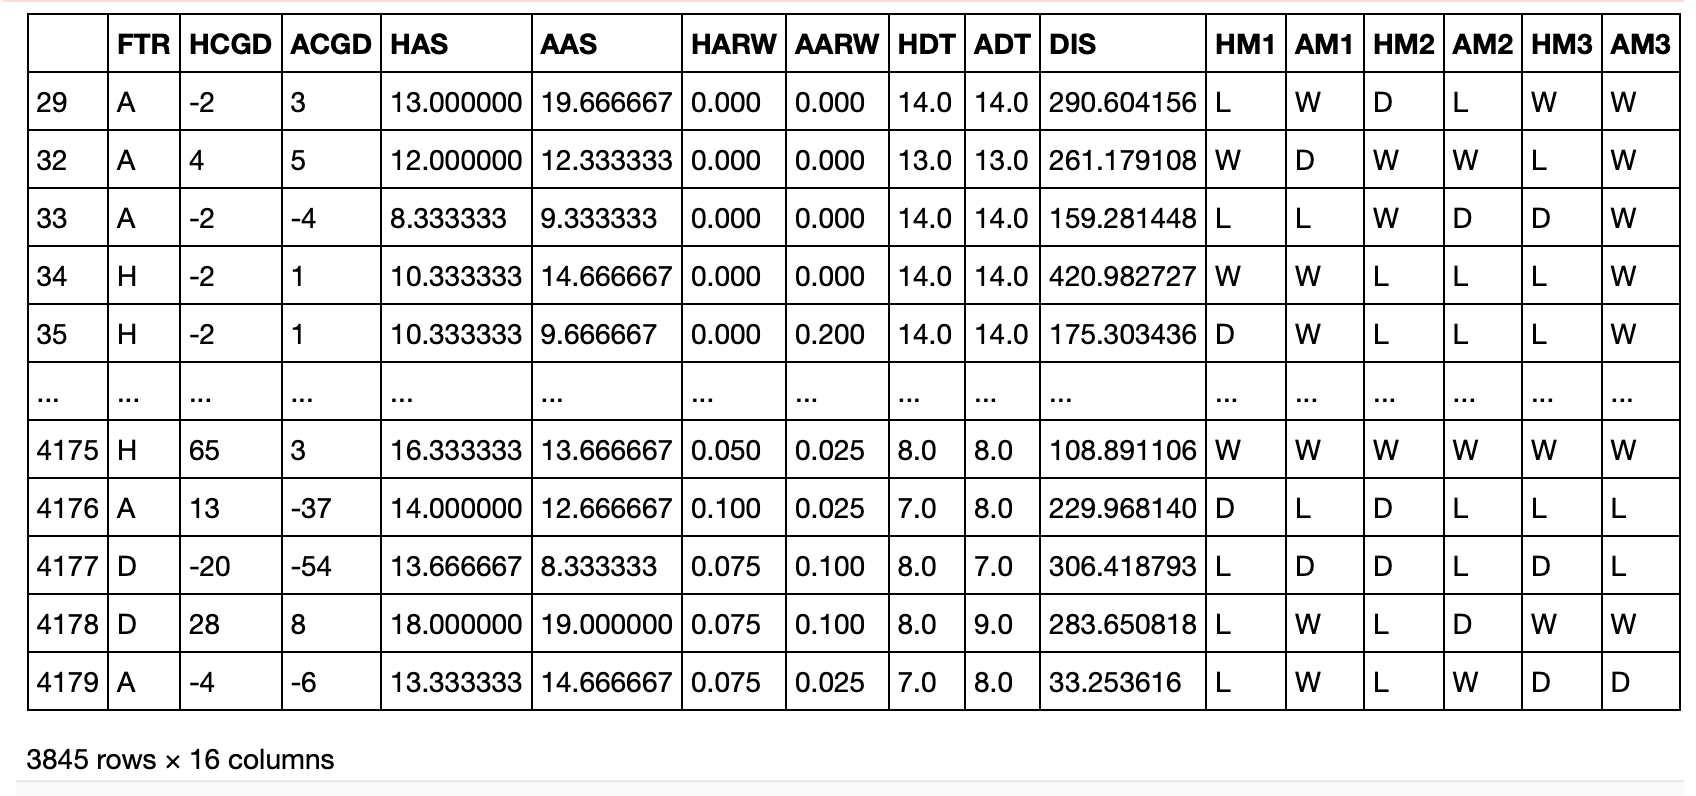
\includegraphics[scale=0.5]{graphs/featureSetWithLabel.png}
\caption{Feature set with one label column}
\label{fig:featureSetWithLabel}
\end{figure}

% -------------------------------------------------------
\subsection{Second Data Exploration - Analyse Numerical Features}
To learn the characteristics of each feature, we derived the minimum, maximum, median, mean, variance and standard deviation:
\begin{figure}[H]
\centering  
\subfigure[]{
\label{Fig.sub.3}
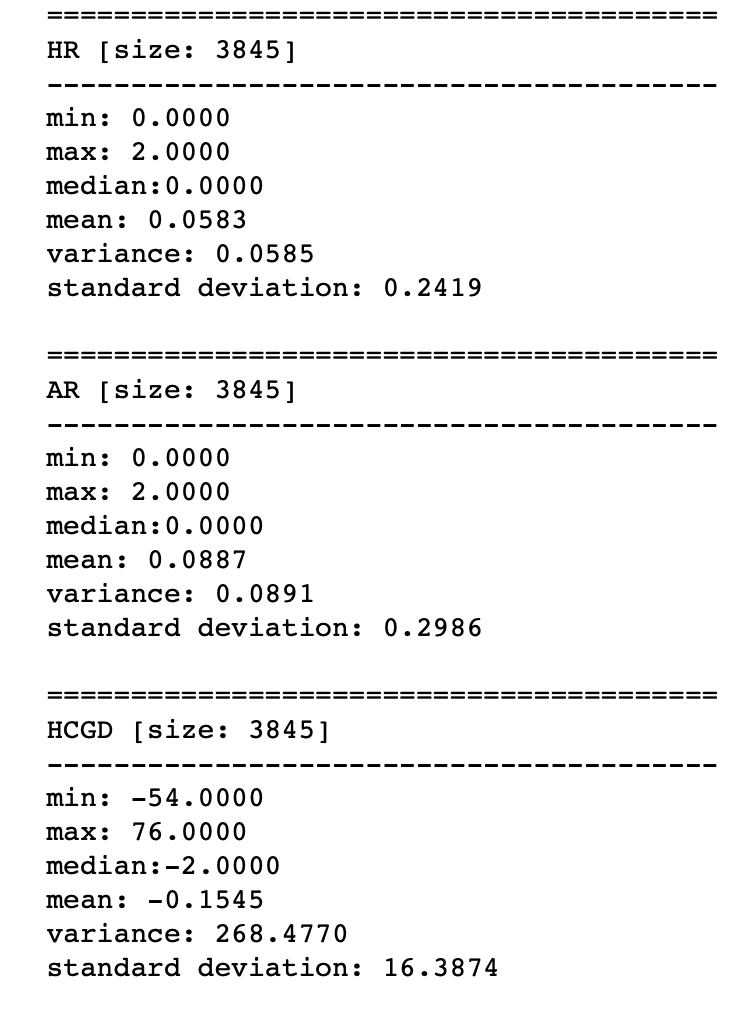
\includegraphics[width=0.32\textwidth]{graphs/statistics1.png}}
\subfigure[]{
\label{Fig.sub.4}
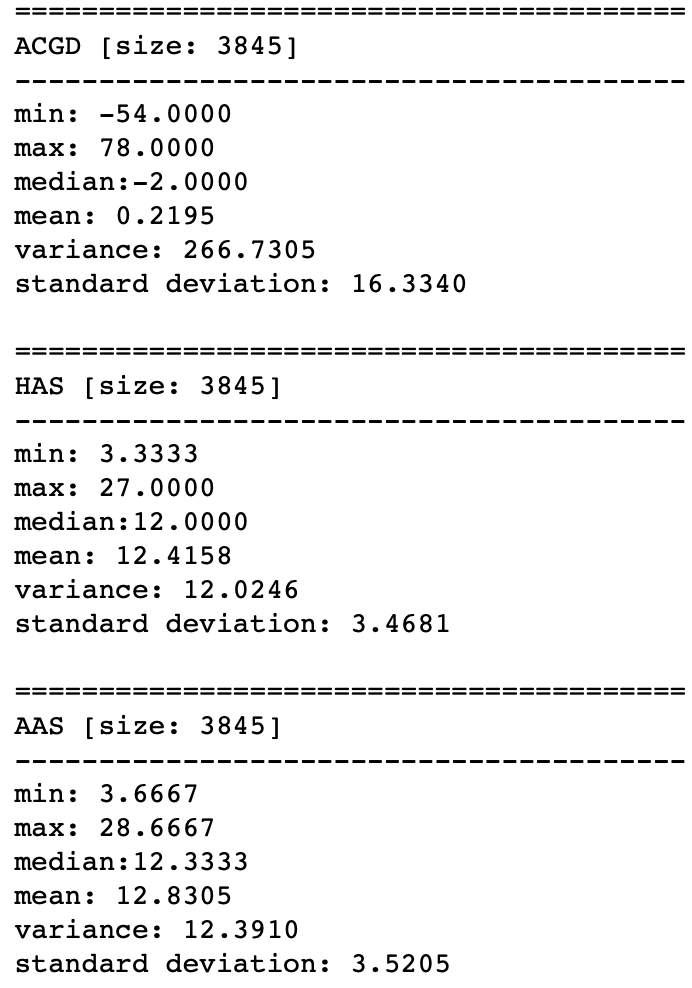
\includegraphics[width=0.32\textwidth]{graphs/statistics2.png}}
\subfigure[]{
\label{Fig.sub.5}
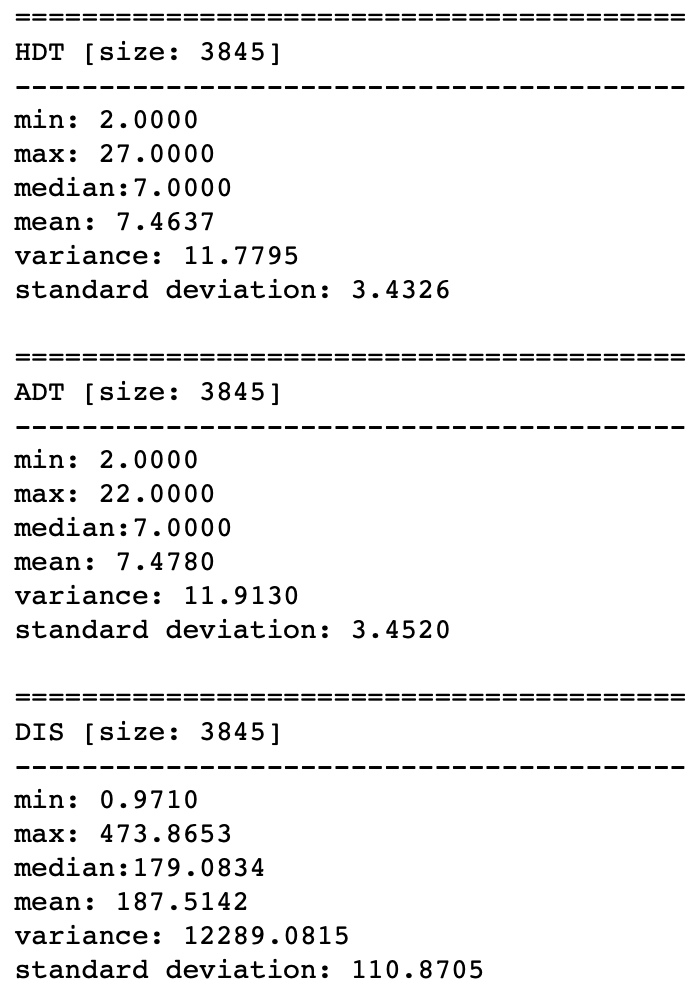
\includegraphics[width=0.32\textwidth]{graphs/statistics3.png}}
\caption{ Statistics of each feature column}
\label{fig:statistics}
\end{figure}

From the figure, we can draw such conclusions:
\begin{itemize}
\item HARW \& AARW: The range is very small (around 0.5). Comparing to the other features, the values of these two are too small.
\item HCGD \& ACGD: Large range (> 130) with negative values involved. The median and the mean demonstrates that there is a relatively greater number of negative values within the data set.
\item AAS \& AAS: Moderate range (around 25) with all positive values. The median and the mean is at the half of the range while the variance is reasonable.
\item HDT \& ADT: Similar moderate range (around 25) and variance with the above pair of data. But the median and the mean is at the one third of the range. Outliers may exist.
\item DIS: Large range (> 450) with all positive values. Reasonable median and mean. But from the variance we can know that the value fluctuates significantly. Comparing to the others, the value is too large.HARW
\end{itemize}

% -------------------------------------------------------
\subsection{Data Transformation}
% --------------------------------------
\subsubsection{Label mapping}
We mapped the label (i.e., FTR) into numbers for later model training by the rule:
\begin{itemize}
\item 'H' $\to$ 1
\item 'A $\to$ 0
\item 'D' $\to$ 2
\end{itemize}

% ------------------------------------
\subsubsection{Rescale and standardize numerical features} \label{`}
With the conclusions from 3.3, we applied the z-score standardization and min-max rescaling to the numerical features.
% -----------------------------------
\subsubsection{Transform categorical features}
The categorical data within the feature set is: \\\\
		\centerline{HM1,AM1, HM2,AM2, HM3,AM3, }\\\\
which only take the values {‘W’, ‘L’, ‘D’}.

So we introduced the binary features		\\\\
\centerline{HM1\_W, HM1\_L, HM1\_D}	\\\\
\centerline{AM1\_W, AM1\_L, AM1\_D}		\\\\	
\centerline{......}		\\\\
\centerline{AM3\_W, AM3\_L, AM3\_D}		\\\\
such that if, for example, HM1 takes the value of ‘W’,  then HM1\_W = 1, HM1\_L= 0, HM1\_D = 0. 

% -------------------------------------------------------------------------------------------
\section{Methodology Overview}
This section will explain what additional data set have we used. Followed by a brief introduction of some base classifiers we applied. After that, we will discuss what techniques that optimize the performance of classifiers have we used. 
%The documentation for \verb+natbib+ may be found at
%\begin{center}
  %\url{http://mirrors.ctan.org/macros/latex/contrib/natbib/natnotes.pdf}
%\end{center}
%Of note is the command \verb+\citet+, which produces citations
%appropriate for use in inline text.  For example,
%\begin{verbatim}
  % \citet{hasselmo} investigated\dots
%\end{verbatim}
%produces
%\begin{quote}
 % Hasselmo, et al.\ (1995) investigated\dots
%\end{quote}

%\begin{center}
  %\url{https://www.ctan.org/pkg/booktabs}
%\end{center}

\subsection{Data set}

Firstly, we add a feature DIS, which is the distance between the stadiums of the two teams. This is done by using a library 'geopy' which allowed us to estimate the distance of latitude and longitude of the city. Besides, we found the stadium location data from \url{https://github.com/jokecamp/FootballData/blob/master/other/stadiums-with-GPS-coordinates.csv}. Although it does not cover every team that appears in the provided data set, we did manage to add missing data manually.

Other features were derived from origin training data. For example, HTdd, home team date delta, means the time between the current match and the previous match of the home team. 

%\begin{figure}
 % \centering
%  \fbox{\rule[-.5cm]{4cm}{4cm} \rule[-.5cm]{4cm}{0cm}}
%  \caption{Sample figure caption.}
%  \label{fig:fig1}
%\end{figure}

\subsection{Base model}
In this problem, we need to classify match result(FTR) into three categories, so we need to build a multi-class classification model to achieve our goal. Hence we found several classic classification models that are suitable for this problem: Multinomial Logistic Regression, Gaussian Naive Bayes, Linear Discriminant Analysis(LDA), Quadratic Discriminant Analysis(QDA), Decision Tree Classifier, and Multilayer Perceptron(MLP, a class of feedforward artificial neural network). These classifiers can be directly imported from Scikit-learn library, and detailed information of these classifiers can be found at:  \url{https://scikit-learn.org/stable/modules/multiclass.html}

\subsection{Model evaluation}
\subsubsection{F1-score}
After the first step, we need to evaluate and optimise our model. As a result, we need to find an evaluation standard for our classifiers. We use f1-score as an analysis of the accuracy of the classification model. \\
The result will be sorted into the matrix. For example, if a result is predicted as false, but the actual result is positive, it will be regarded as TN. 
\begin{figure}[ht]
\centering
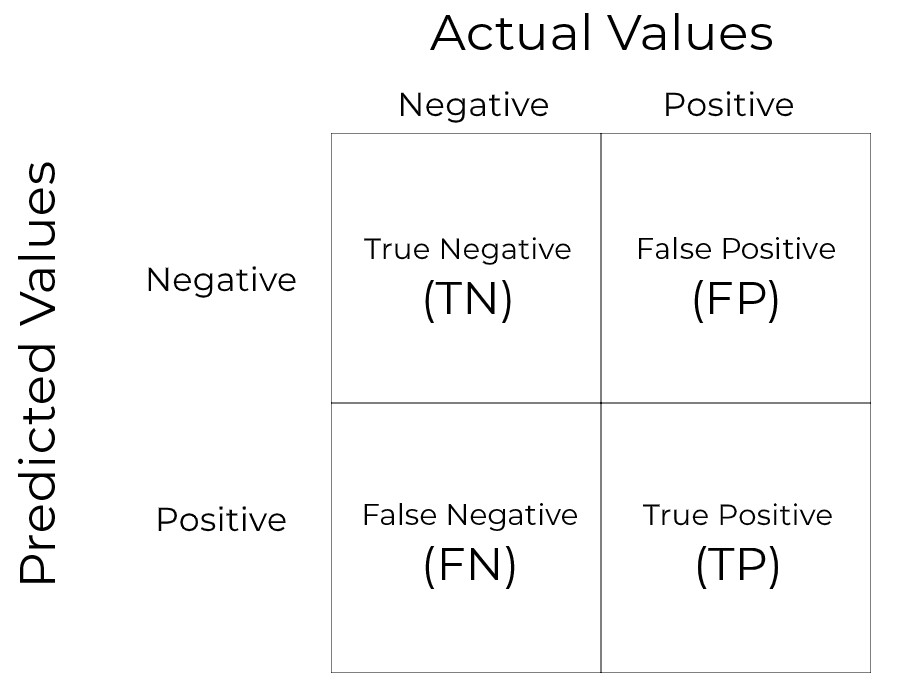
\includegraphics[scale=0.2]{graphs/confusion_matrix.jpeg}
\caption{Confusion Matrix\cite{6}}
\label{fig:confusion_matrix}
\end{figure}

After that, the f1-score is calculated from precision(\( p\)) and recall(\(r\)), where:
\begin{equation}
p = \frac{TP}{TP+FP}\\
\end{equation}
\begin{equation}
r = \frac{TP}{TP+FN} \\
\end{equation}
\begin{equation}
f1\_score = 2*\frac{p*r}{p+r}\\
\end{equation}

It shows that f1-score indicates both precision and recall of a model, while accuracy can be contributed mainly by a large number of True Negatives. In this case, f1-score might be a better measure to use since we need to seek a balance between Precision and Recall\cite{1}

\subsubsection{Cross-Validation}
Cross-Validation split training set into several folds, then train the model using all folds but one as a training set each time. The remaining folds will be regarded as a validation set. \\
Cross-Validation allows us to perform validation, but still maintaining the training data set. Thus it will reduce overfitting.

\subsubsection{Parameter optimization}
A model has many parameters, and diverse parameters produce different model performance. So we need to define a range of parameters to be adjusted for each model and find an approach to seek the best model(with highest f1-score).
 
\subsubsection{Ensemble methods}
Ensembled methods seek to consolidate the predictions of one or more base models built with a specific learning algorithm in order to improve the performance of a single model.

There are two main classes of ensemble methods, which are averaging method and boosting method. The averaging method looks to build several classifiers independently and average their predictions while in boosting methods, base estimators are built sequentially, and one tries to reduce the bias of the combined estimator.

Initially, we intended to use a bagging classifier(an averaging method). However, we found from Vu, Braga-Neto, and Dougherty \cite{4}that an empirical basis that ensemble classification by bagging cannot increase the performance of stable classification rules, such as linear discriminant analysis. It seems bagging methods were not a fitting model in this case. As a result, we decide to use boosting methods instead. Based on research by Martínez-Muñoz\cite{3}, Marina and Robert P W\cite{2}, it seems LDA and NN can be theoretically used as the base estimator in boosting model.

% -------------------------------------------------------------------------------------------
\section{Model Training \& Validation}
In this section, we created groups of parameters to be optimised for each base model, and then we got six optimised classifier with parameters that has the best f1-score. We also applied cross-validation and generate a cross-validation-score for each model as well. Next, we used them as base-estimator in boosting methods. Finally, we compared the overall performance based on f1-score and cross-validation-score and presented the best estimator.

\subsection{Optimization of base estimator}

\subsubsection{Cross-Validation}
KFold function was used to split the training data into ten sets.We use model\_selection.cross\_val\_score function, it generates a cross-validation score for a model based on the given model and k folds. 

\subsubsection{Parameter optimisation}
A model has many parameters in it. However, we cannot optimse all of them since that will take a massive amount of time to compute. So we select several parameters that could potentially affect the most.
After we specified a group of parameters for each model, we then pass that as a parameter to train\_predict function together with an f1-scorer. It will use GridSearchCV function to choose parameter with the highest f1-score and produce the best estimator. 

\subsection{Result}
Now we get the result of the prediction on test set by the six optimised models which is shown below:\\
\begin{figure}[ht]
\centering
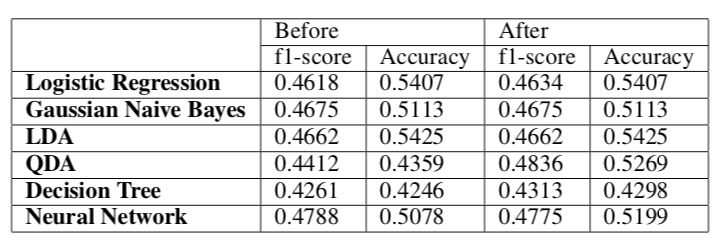
\includegraphics[scale=1]{graphs/result_table.png}
\caption{Parameter optimisation result}
\label{fig:confusion_matrix}
\end{figure}

We noticed LDA seems do not change after optimisation, and this could because the parameter group we selected is not large enough, or the default model is already relatively optimised. However, after we tried different possible parameters(some of the parameters are not supported under some particular condition like shrinkage is not supported when the solver is "svd") and increase the range of parameter selection, the result still did not change. So we supposed we could consider the origin setting to be approximately optimised.

In addition, the f1-score of NN slightly decreased  after optimisation, and this could because there was some error during fitting or it was slightly overfitted. 

In general, the performance of most of the models slightly increased after optimisation. This means our optimisation is valuable. 

\subsection{Ensemble methods}
\subsubsection{Ada boost}
We used AdaBoostClassifier from scikit-learn as an ensemble method. An AdaBoost classifier is a meta-estimator that starts by fitting a classifier on the original training set and then fits additional copies of the classifier on the same training set but where the weights of incorrectly classified instances are adjusted such that subsequent classifiers focus more on difficult cases.\cite{5}

It allows using a single classifier as a base estimator so that we can feed our optimised classifier into it. However, there is some pre-condition to be the base estimator. First, it must provide the "predict\_proba" method, which is not supported by QDA and LDA. We tried implementing the function ourselves and switching algorithms in AdaBoostClassifier, but none of them worked. As a result, we have to give up feed LDA and QDA in ensemble methods. 

MLP classifier is not supported as well, but we do find an approach to implement the missing attribute in MLP classifier. It now works after we implemented customMLPClassifier class, although the run time for that is remarkably long. We found this solution from: \url{https://stackoverflow.com/questions/55632010/using-scikit-learns-mlpclassifier-in-adaboostclassifier}

Moreover, we tried to optimise parameter of the AdaBoostClassifier as well. However, it will take forever to compute. So we dropped this task for this classifier.

\subsubsection{Gradient boost}
We also found another classifier provided called GradientBoostClassifier. It builds an additive model in a forward stage-wise fashion. it allows for the optimization of arbitrary differentiable loss functions. In each stage n\_classes regression trees are fit on the negative gradient of the binomial or multinomial deviance loss function. \cite{5}

There is no base\_estimaor parameter in GradientBoostClassifier. It only has loss as a parameter, which is the loss function, and it can take two values: deviance and exponential. Fortunately, the deviance option is the same with Logistic regression so that we can regard it as a kind of ensemble model on the Logistic Regression classifier.

\subsubsection{Ensemble methods result}
The result is shown below:\\
\begin{figure}[ht]
\centering
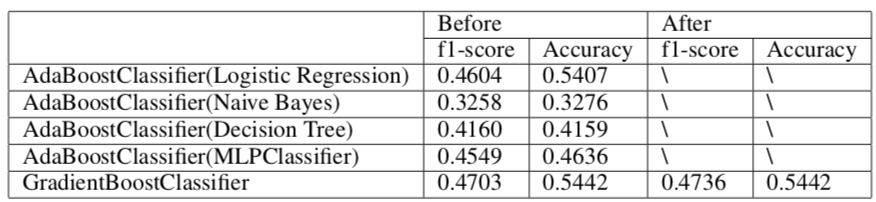
\includegraphics[scale=1]{graphs/ensemble_result_table.png}
\caption{Ensemble methods result}
\label{fig:confusion_matrix}
\end{figure}\\
We did not do parameter optimisation for AdaBoostClassifier(run-time problem), so the After column is empty. We noticed that the performance of AdaBoostClassifier with Naive Bayes, Decision Tree, and MLP Classifier is worse than that of a single classifier. Another unusual thing here is that AdaBoostClassifier with MLPClassifier as a base estimator has f1-score and accuracy of over 70 when predicting from the training set. It could be evidence of overfitting.
\subsection{Final model}
After combining all the results, we noticed that accuracy score of GradientBoostClassifier(after parameter optimisation) is the highest among 11 classifier we tested. Although the f1-score is slightly lower than that of QDA(-0.01) and Neural Network(MLP Classifier)(-0.029), the accuracy is much more higher(+0.0173 and + 0.0243). So we think GradientBoostClassifier is the most suitable model in this case.
%\begin{table}[]
%\centering
%\begin{tabular}{|l|l|l|l|l|}
%\hline
 %                                       & \multicolumn{2}{l|}{Before} & \multicolumn{2}{l|}{After}          \\ \cline{2-5} 
  %                                      & f1-score     & Accuracy     & f1-score         & Accuracy         \\ \hline
%AdaBoostClassifier(Logistic Regression) & 0.4604       & 0.5407       & \textbackslash{} & \textbackslash{} \\ \hline
%AdaBoostClassifier(Naive Bayes)         & 0.3258       & 0.3276       & \textbackslash{} & \textbackslash{} \\ \hline
%AdaBoostClassifier(Decision Tree)       & 0.4160       & 0.4159       & \textbackslash{} & \textbackslash{} \\ \hline
%AdaBoostClassifier(MLPClassifier)       & 0.4549       & 0.4636       & \textbackslash{} & \textbackslash{} \\ \hline
%GradientBoostClassifier                 & 0.4703       & 0.5442       & 0.4736           & 0.5442           \\ \hline
%\end{tabular}
%\end{table}


% -------------------------------------------------------------------------------------------
\section{Results }

In the application of machine learning model, the prediction of result is the black-box process. Therefore, human cannot understand the prediction from model without corresponding explanation, so the optimization of model becomes harder, either.

To achieve that, LIME, an open-source tool to explain the machine learning models, is used to analyse final result. 

\subsection{Introduction of LIME}
In order to explore the behaviors of models, LIME will perturb the input to approximate the black-box model by a simple interpretable one. It means the explanation can cover most of samples but not all of them.\\

There is an example about how LIME explaining the model (Fig.\ref{fig:LIMEintro}):

\begin{figure}[ht]
\centering
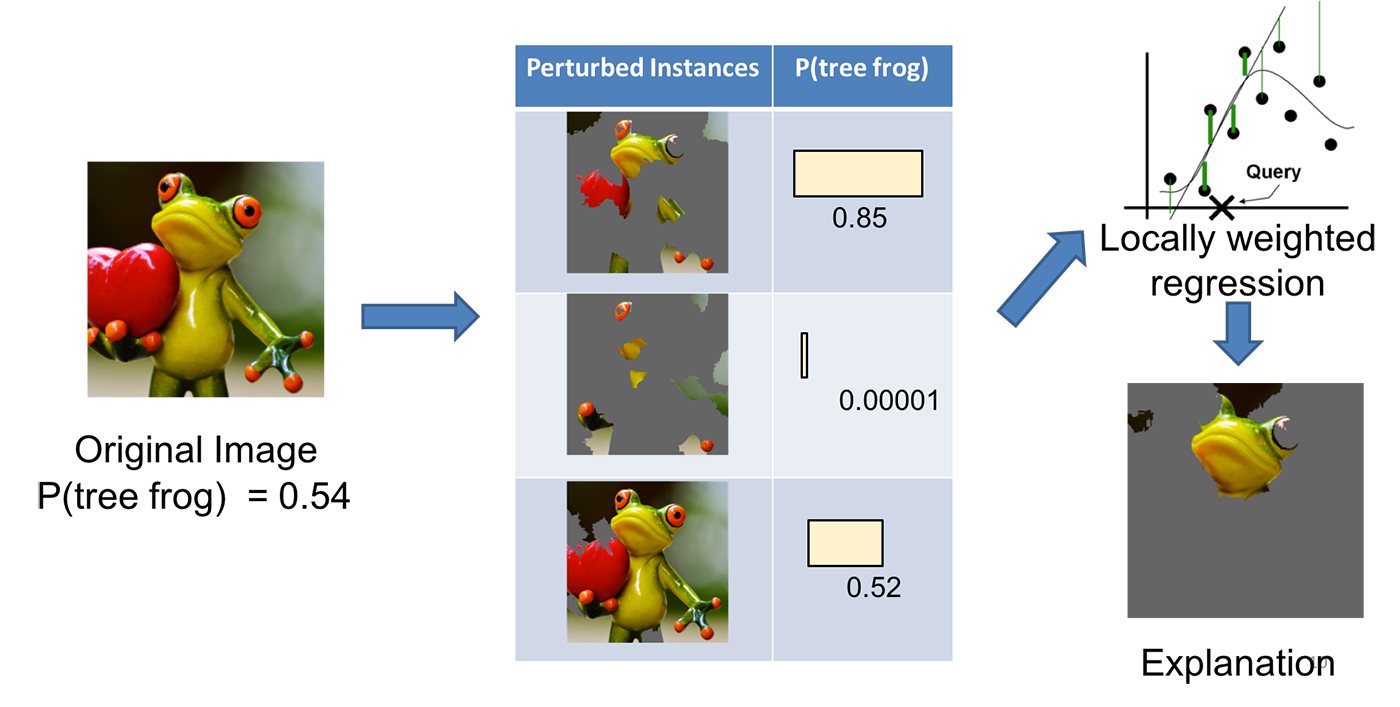
\includegraphics[scale=0.4]{graphs/LIMEintro.png}
\caption{}
\label{fig:LIMEintro}
\end{figure}

\subsection{Explanation of Samples}
To understand the trained model, we will take these 3 matches as samples (Fig.\ref{fig:LIMEsample}):

\begin{figure}[ht]
\centering
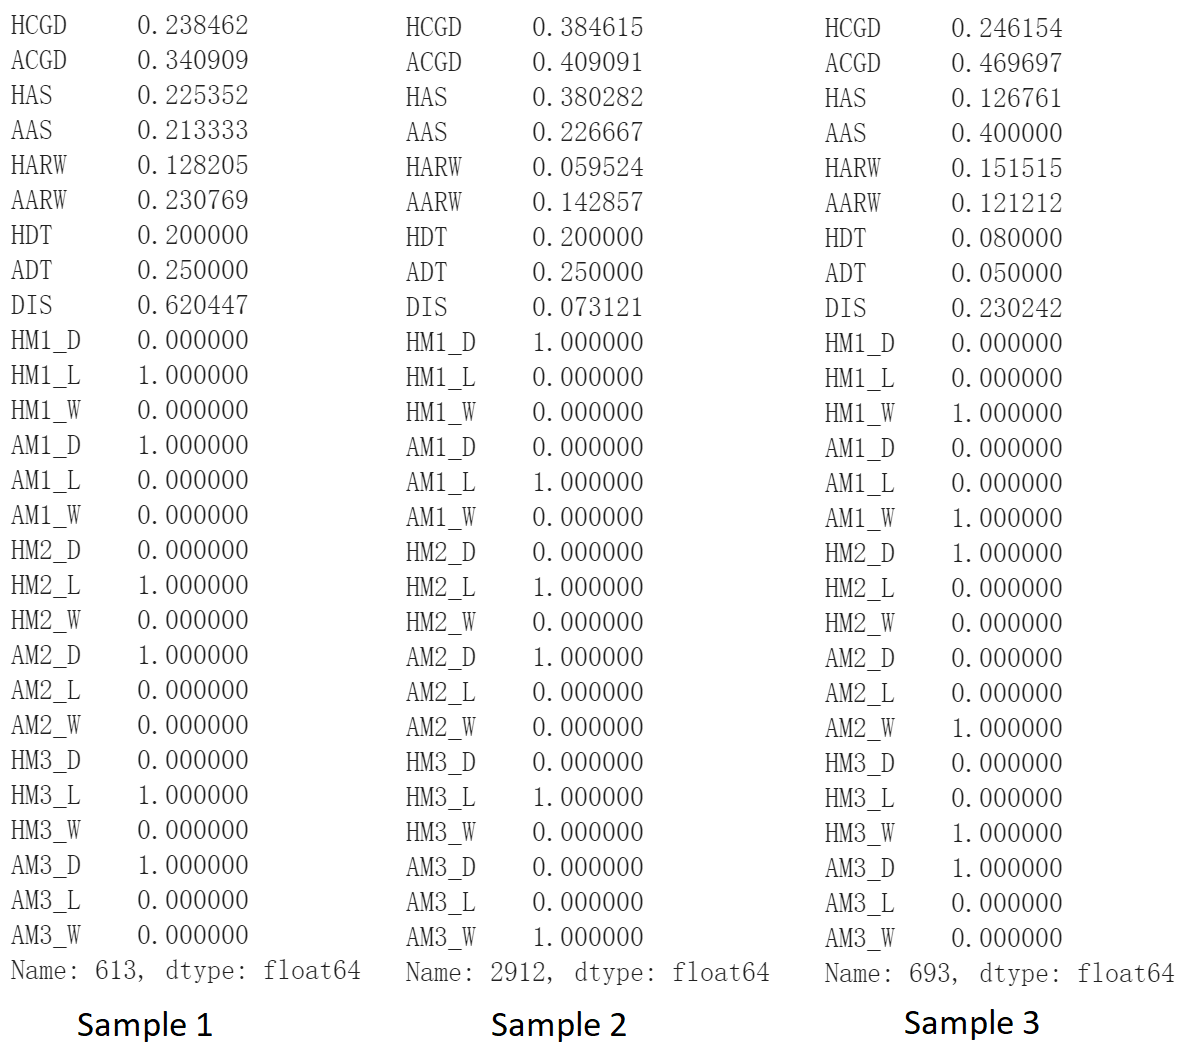
\includegraphics[scale=0.7]{graphs/LIMEsample.png}
\caption{}
\label{fig:LIMEsample}
\end{figure}

For the explainer, it shows the five top features which influence the prediction of final results.

The explanations of results are shown in Fig.\ref{fig:LIMEresult}.

\begin{figure}[ht]
\centering
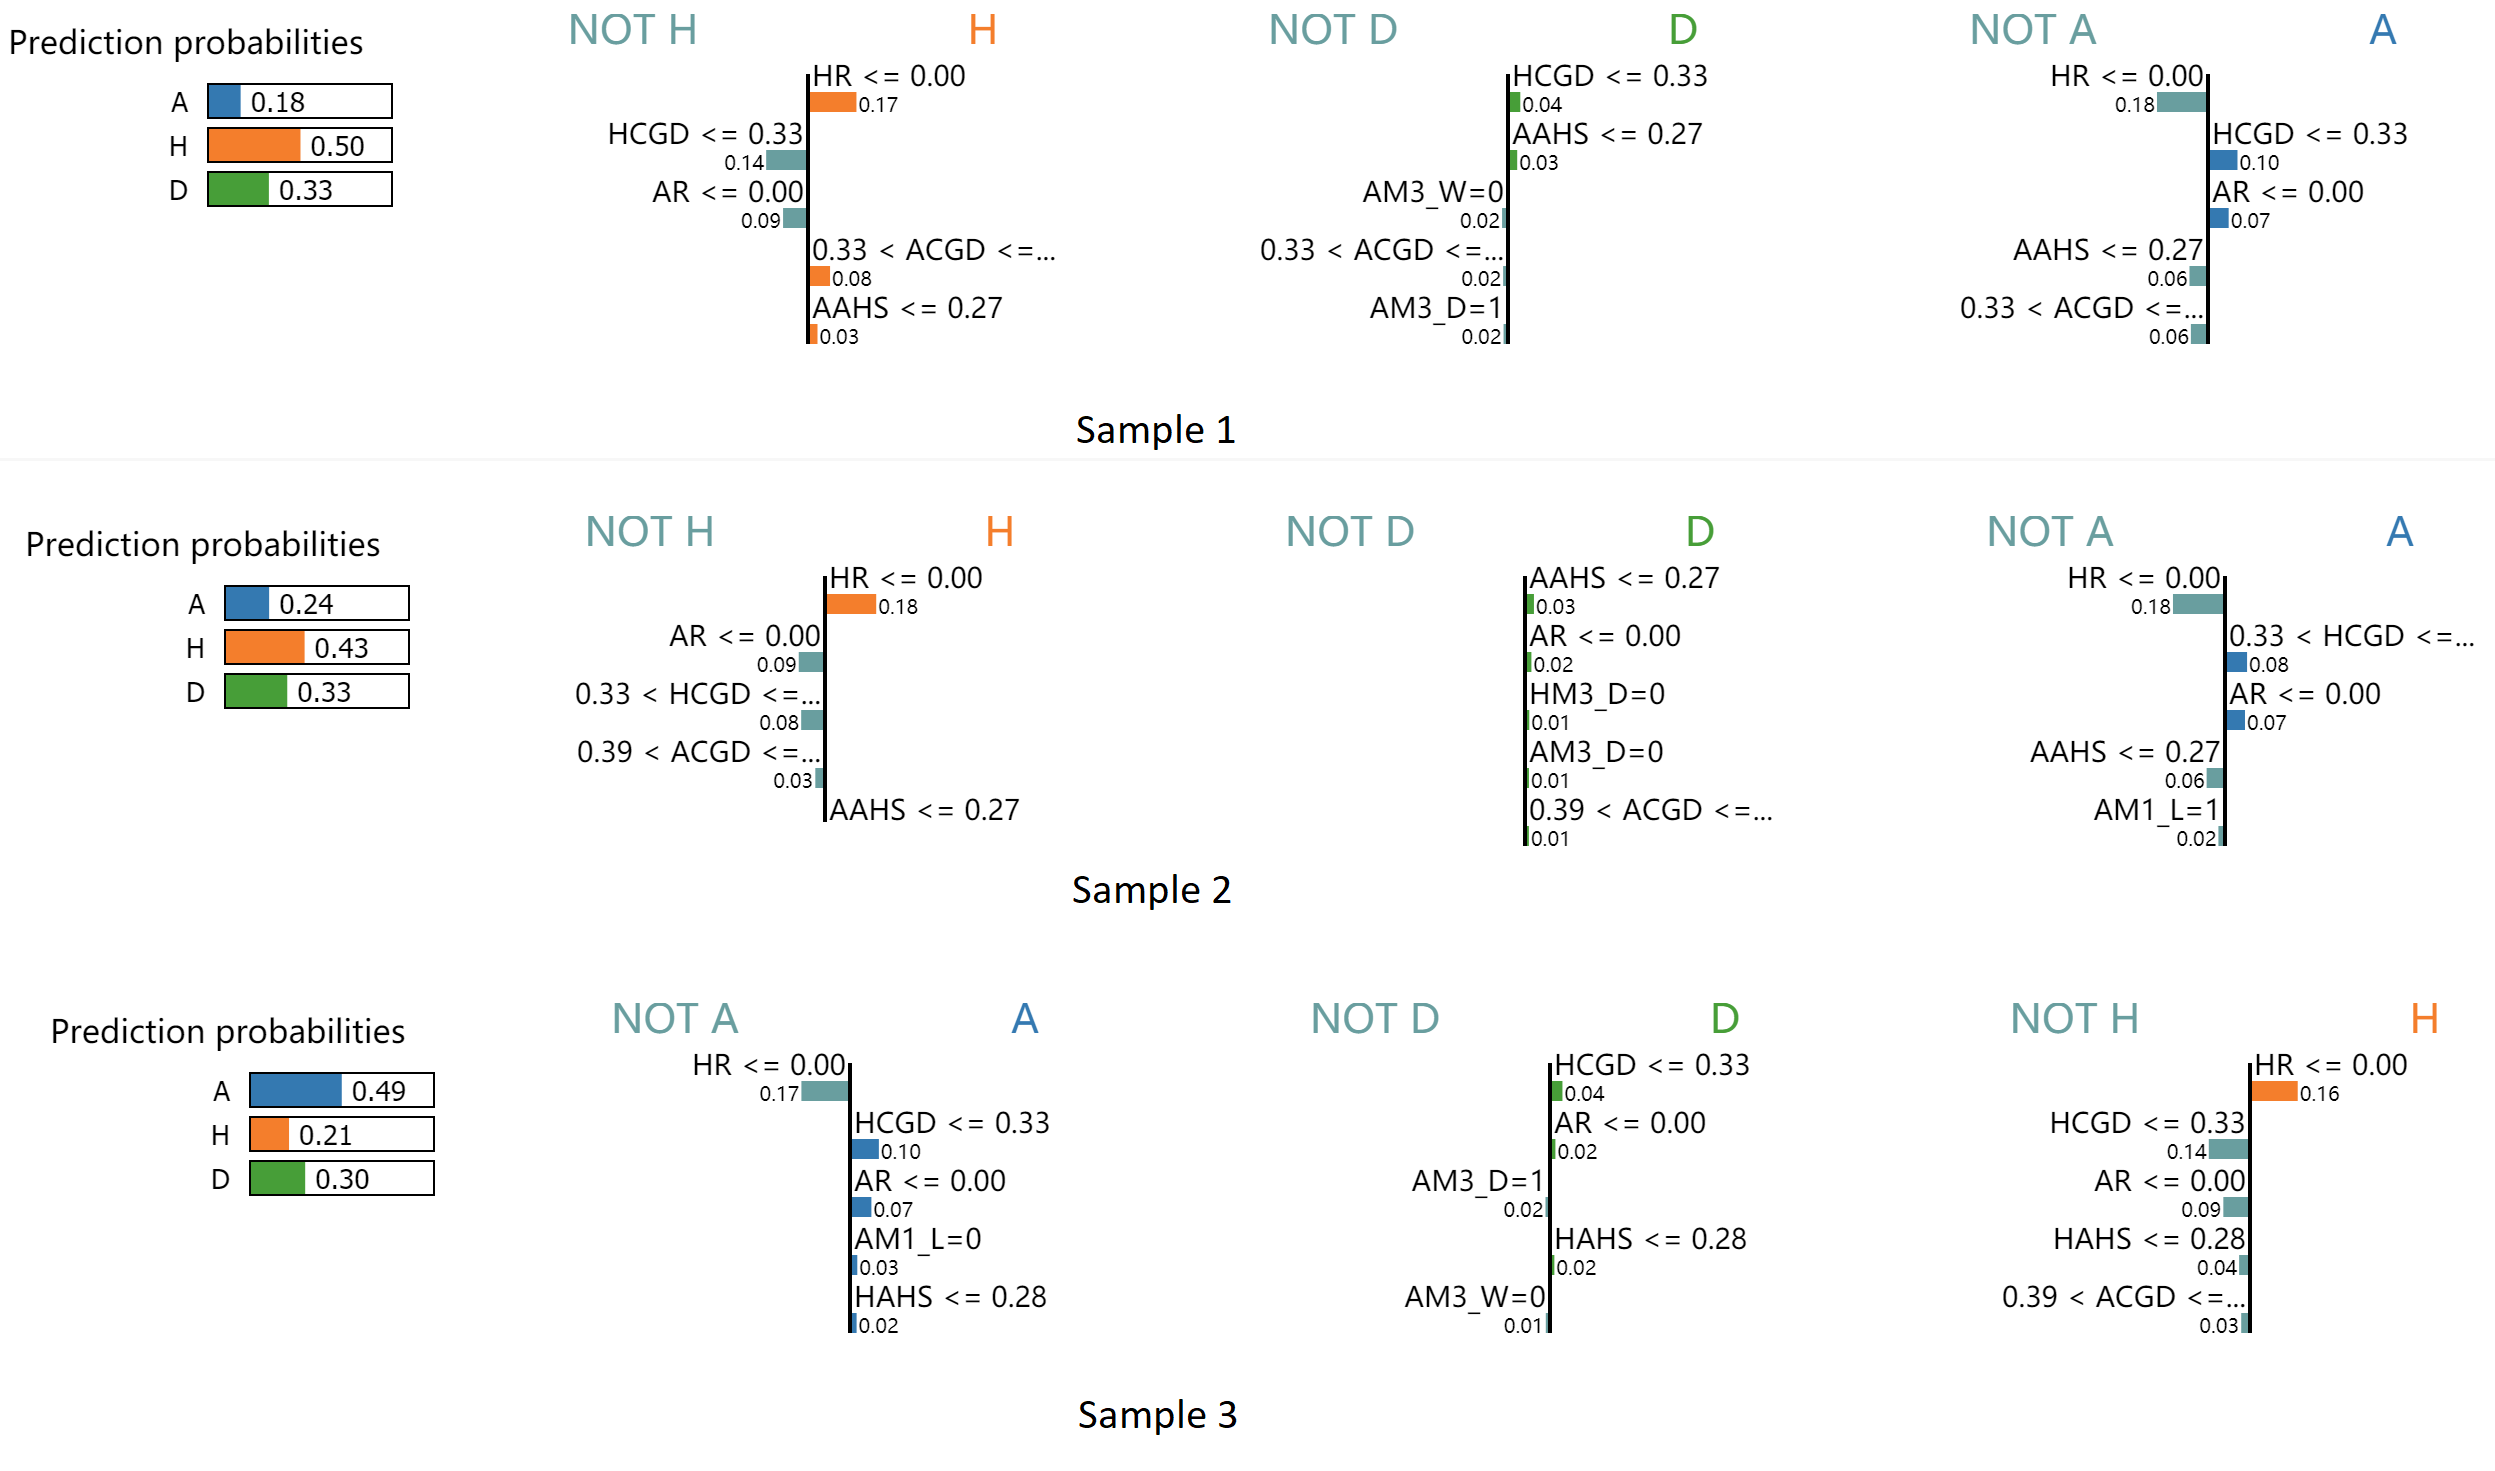
\includegraphics[scale=0.4]{graphs/LIMEresult.png}
\caption{}
\label{fig:LIMEresult}
\end{figure}

\subsection{Analysis \& Insights}
As shown above, there are three possible results: H (HomeTeam win), A (AwayTeam win) and D (Draw). For each result, classifier takes different features as  evaluation criterion:
\begin{itemize}
\item[-] For H/Not H and A/Not A, this classifier takes HR (Average number of red cards received by the home team in nearly matches) as the most significant feature to determine the winning percentage of home team. In the other words, if a home team did not get any red cards in the matche, on average, the winning rate of home team would be about 0.17 higher. 

From the rules of football match, if a football player get a red card, he will not be permitted to take furthur part in the game, this can be regarded as an disadvantage in matches.\\

\item[-] Similarly, AR (Average number of red cards received by the away team in nearly matches) also plays an important role in final results. However, comparing with HR, AR has less effect on final results. The reason for that need to be carefully discussed in future. 

\item[-] As an essential feature representing the player's capability of home team, HCGD (the cumulative full-time goal difference by home team) cannot be neglected, either. The rise of HCGD can effectively increase the possibility of hometeam-win.

In the other side, ACGD (the cumulative full-time goal difference by away team) does not have clear relationship with final results.

\item[-] The possibility of Draw is related to a number of factors, such as AR, HCGD, and AHS. Nevertheless, each one of them does not have more impact on final results than others. The explanation of these 3 samples illustrates that Draw might be a coincident to some extent under particular situation.

\item[-] This explanation also reveal that HDT/ADT (the delta time from last match of home team and away tea) and DIS (distance between two teams) have little effect on results. 

\end{itemize}

% -------------------------------------------------------------------------------------------
\section{Final Predictions on Test Set}
% -------------------------------------------------------
\subsection{Data Pre-processing}

Before predicting the result we first need to process the test set to fit our model. We applied similar operations as we dealing with the training data. To derive features, we import the up-to-date data of the season 2019 from {\em<http://www.football-data.co.uk>} .

Our prediction is shown in the Fig.\ref{fig:finalPrediction},
\begin{figure}[ht]
\centering
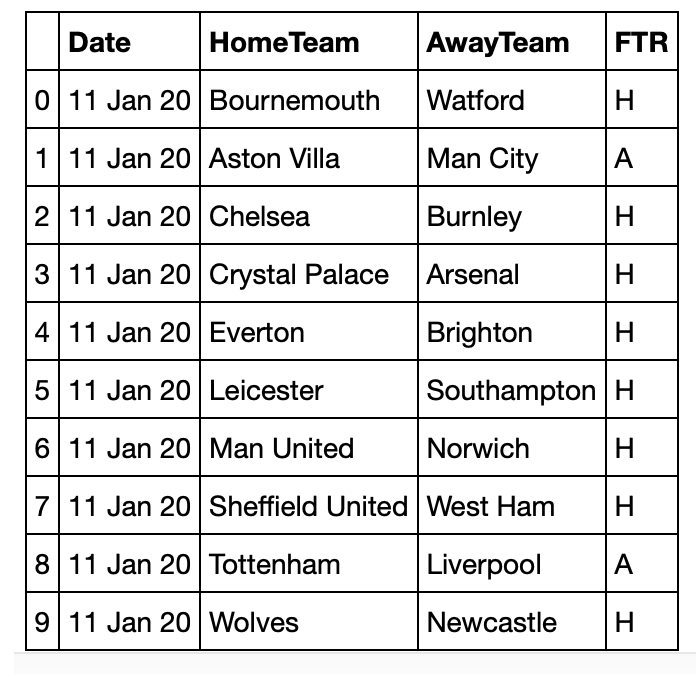
\includegraphics[scale=0.5]{graphs/finalPrediction.png}
\caption{Final prediction}
\label{fig:finalPrediction}
\end{figure}

% -------------------------------------------------------------------------------------------
\section{Conclusion [Terry]}




% -------------------------------------------------------------------------------------------
\bibliographystyle{unsrt}  
%\bibliography{references}  %%% Remove comment to use the external .bib file (using bibtex).
%%% and comment out the ``thebibliography'' section.


%%% Comment out this section when you \bibliography{references} is enabled.
\begin{thebibliography}{1}


\bibitem{1}
Brownlee, Jason
\newblock (2014)
\newblock Classification Accuracy is Not Enough: More Performance Measures You Can Use
\newblock {\em<https://machinelearningmastery.com/classification-accuracy-is-not-enough-more-performance-measures-you-can-use>}.

\bibitem{2}
Marina Skurichina; Robert P. W. Duin
\newblock (2000)
\newblock Boosting in Linear Discriminant Analysis - Multiple Classifier Systems
\newblock P.190-199
\newblock Publisher: Springer Berlin Heidelberg
\newblock Dec 1st 2000
\newblock ISBN: 978-3-540-45014-6
\newblock {\em<https://arxiv.org/abs/1909.12098v1>}.

\bibitem{3}
Martínez-Muñoz, Gonzalo
\newblock (2019)
\newblock Sequential Training of Neural Networks with Gradient Boosting
\newblock Sep 26th  2019
\newblock {\em<https://arxiv.org/abs/1909.12098v1>}.

\bibitem{4}
Thang T. Vu ; Ulisses M. Braga-Neto ; Edward R. Dougherty
\newblock (2019)
\newblock Bagging degrades the performance of linear discriminant classifiers
\newblock July 24th 2009
\newblock Published in: 2009 IEEE International Workshop on Genomic Signal Processing and Statistics
\newblock DOI:10.1109/GENSIPS.2009.5174344
\newblock {\em<https://ieeexplore.ieee.org/document/5174344>}.

 \bibitem{5}
Scikit-learn
\newblock (2019)
\newblock 1.11. Ensemble methods
\newblock {\em<https://scikit-learn.org/stable/modules/ensemble.html\#ensemble>}.

\bibitem{6}
Radečić, Dario 
\newblock (2009)
\newblock A Non-Confusing Guide to Confusion Matrix
\newblock Sep 28th 2009
\newblock {\em<https://towardsdatascience.com/a-non-confusing-guide-to-confusion-matrix-7071d2c2204f>}.
 

\bibitem{sharma}
Sharma, Mohit.
\newblock What Steps should one take while doing Data Preprocessing?.
\newblock June 20th 2018.
\newblock June 1st 2019.
\newblock {\em<https://hackernoon.com/what-steps-should-one-take-while-doing-data-preprocessing-502c993e1caa>}.

\bibitem{gonz}
J. González.
\newblock Scaling/ normalisation/ standardisation: a pervasive question.
\newblock Oct 18th 2018.
\newblock June 3st 2019.
\newblock {\em<https://quantdare.com/scaling-normalisation-standardisation-a-pervasive-question/>}.
  

\end{thebibliography}


% -----------------------------------------------------------------------------------------
\end{document}